\documentclass[12pt]{article}

\usepackage{graphicx}
\graphicspath{ {Fichier_Image/} }

\title{10 Premiers Bâtiments}
\author{Thibault Clodion}

\begin{document}

\maketitle % Permet d'afficher le titre, l'author etc

\section{Type de Batiments}

\begin{enumerate}

\item Couloir 1 m
\item Couloir 1.50 m
\item Couloir sans limite
\item 5 Personnes max par bureau
\item 10 Personnes max par bureau
\item 20 Personnes max par bureau
\item 30 Personnes max par bureau
\item 1 Porte par bureau
\item 2 Porte par bureau 
\item 3 Porte par bureau

\end{enumerate}

\underline{Schéma de la forme générale du batiment :}\newline
\includegraphics[scale=0.17]{General Looking.jpg}

\section{Observations}

\begin{enumerate}

    \item Temps moyen de dernière sortie : 24.51 sec
    \newline Temps max de dernière sortie : 28.68 sec
    \newline Temps min de dernière sortie : 21.28
    \newline 
    D'abord après 100 simulations on obtient un temps moyen de sortie étant de 24.55 sec.
    Pour le batiment avec les 250 tables uniformes j'avais un temps moyen de 26.20 sec. C'est donc encourageant
    car cela veut dire que la disposition du bâtiment influe effectivement sur le temps de sortie.
    \newline
    Le bâtiment est un peu vide mais on peut déjà constater plusieurs phénomènes intéressant :
    \newline
    $\hspace*{0.2cm}$- L'important est de \textbf{Diviser le flux} cela permet d'évider les "embouteillages"
    \newline
    $\hspace*{0.2cm}$- Il est aussi important de disposer les tables et bureaux loin des "passages" cela permet
    une arrivée plus rapide vers la sortie sans besoin d'esquiver des meubles
    \newline
    $\hspace*{0.2cm}$- Il est très intéressant d'éloigner les portes entres elles. Car les flux sont importants proches
    des portes, ainsi en les éloignant on s'assure de ne pas réunir deux flux importants et de les garder diviser.
    Je pense donc que la simulation 9 et 10 vont être intéressantes. (pourquoi pas tester une 11ème où les portes sont 
    toujours en face les unes des autres pour illustrer les propos dis ici). 
    \newline
    $\hspace*{0.2cm}$- On peut aussi constater qu'il est intéressant d'avoir des
    murs et des portes car le temps à réduit comparer à la simulation avec 250 tables uniformes, donc on ne peut imaginer un batiment sans mur
    pour optimiser le bâtiment (ceci car cela génère un flux important devant les uniques portes du bâtiments alors qu'il faut diviser le flux).
    \newline
    La photo montre le fait qu'il y a toujours des flux importants à certaines portes. 
    \newline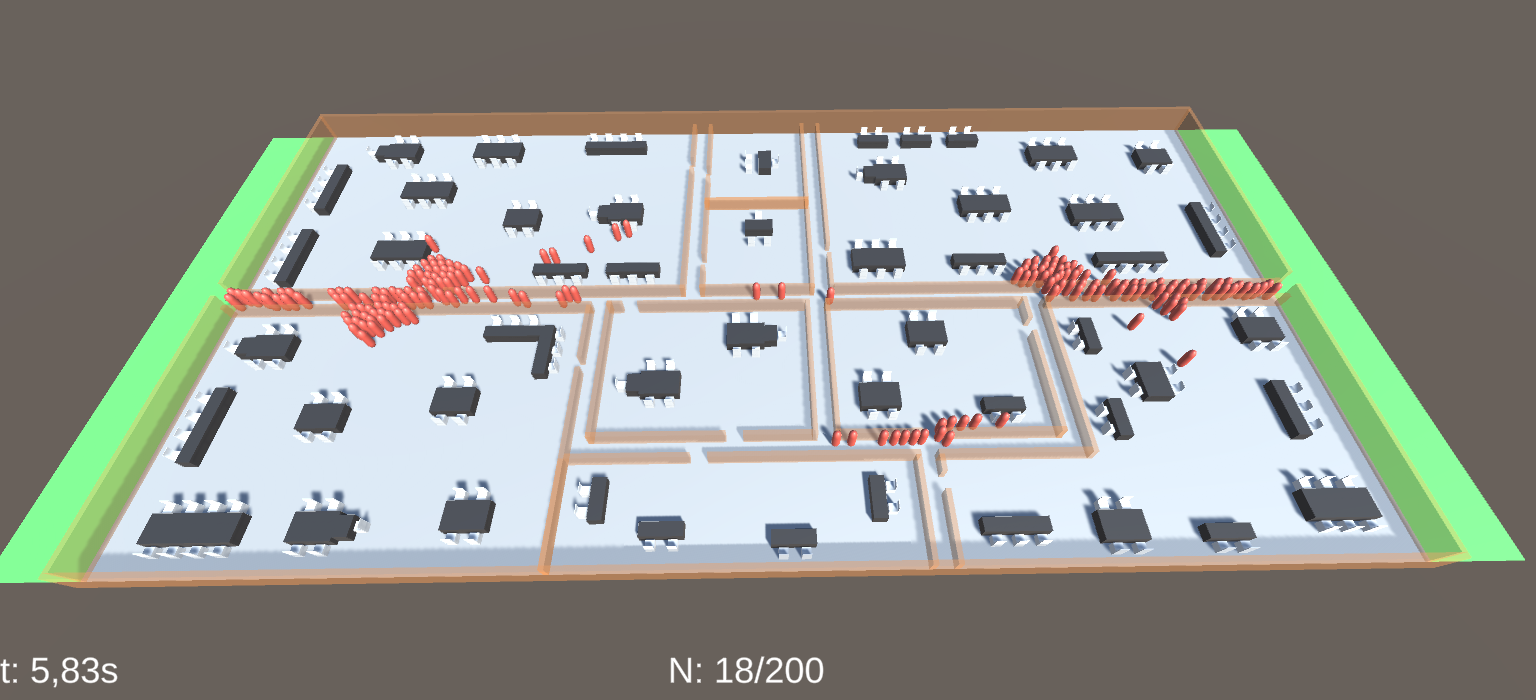
\includegraphics[scale=0.17]{1. couloir 1m -(2).png}
    
    \item Temps moyen de dernière sortie : 28.87 sec
    \newline Temps max de dernière sortie : 33.60 sec
    \newline Temps min de dernière sortie : 24.66
    \newline
    Il est très intéressant de voir qu'augmenter la taille du couloir a finalement eu un effet néfaste sur le temps de sortie
    ceci s'explique par deux facteurs :
    \newline
    $\hspace*{0.2cm}$- Les portes n'ont pas augmenter de taille
    \newline
    $\hspace*{0.2cm}$- Les personnes se retrouvent alors bloqué devant la porte de sortie (il ya génération d'un important flux devant
    les portes de sortie).
    \newline
    Donc il semble important que la taille des portes soit en adéquation avec la taille des couloirs avant de ne pas générer des flux trop important
    ci-dessous on peut voir les flux devant les portes de sorties.
    \newline 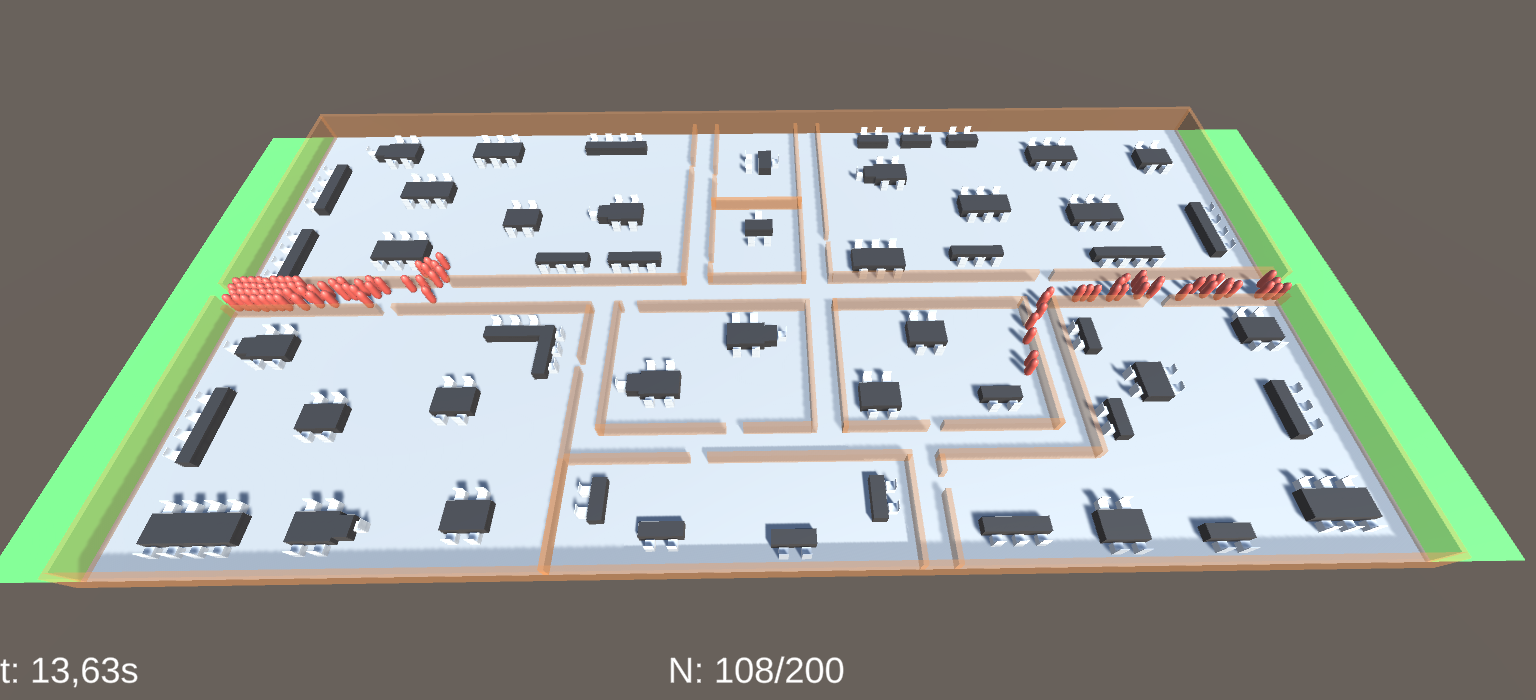
\includegraphics[scale=0.17]{2. couloir 1m50.png}

    \item Temps moyen de dernière sortie : 24.74
    \newline Temps max de dernière sortie : 30.44
    \newline Temps min de dernière sortie : 22.00
    \newline
    Pour ce problème j'ai simplement changer le couloir principal en le repassant à 1m de largeur (soit la largeur de la porte de sortie).
    Ceci étant pour tester si le majeur problème du 2. était le fait qu'il y avait des flux importants devant les portes de sorties du au faite que les couloirs
    était plus grand que les portes. Cependant j'ai laissé les autres couloirs à 1m50 afin de voir si cela avait une influence sur le temps de sortie moyen.
    \newline
    $\hspace*{0.2cm}$- On a toujours les problèmes de flux importants devant les portes (cela bloque la fluidité de l'évacuation)(voir photo du 1.)
    \newline
    $\hspace*{0.2cm}$- Le fait que certains couloirs soit plus grand permet parfois d'acceder plus facilement au couloir principal
    \newline
    $\hspace*{0.2cm}$- Les plus grands couloirs sont peu fréquentés, donc cela ne créer pas plus de bouchon que dans le 1. ce qui peut expliquer le temps de sortie similaire au 1.
    \newline\newline
    Finalement c'est pas forcément utile d'avoir des grands couloirs, cela ne fait qu'ajouter du flux dans d'autres endroits plus restreint, donc cela n'est pas très utile.
    Ce qu'il faut retenir c'est que les couloirs devant les portes ou les endroits "principaux" doivent être de la même taille (c'est à dire que si l'on passe d'un couloir d'1m50 a 1m cela ne fait que créer du ralentissement).
    Donc il peut être compréhensible d'utiliser seulement la taille de la porte pour tous les couloirs. (à voir dans les futures hypothèses)

    \item Temps moyen de dernière sortie : 24.79
    \newline Temps max de dernière sortie : 34.67
    \newline Temps min de dernière sortie : 21.49
    \newline
    J'ai choisi de garder le batiment 1. pour les couloirs étant donné que c'est celui qui a donné le meilleur temps moyen.
    \newline\newline
    $\hspace*{0.2cm}$- Problème lorsque deux personnes aux destinations opposés se retrouvent dans le même couloir face à face (cela fait perdre du temps, le problème vient peut-être de la manière de calculer la porte choisie et 
    du fait qu'aucun n'individu ne change d'avis durant la simulation)
    \newline
    $\hspace*{0.2cm}$-Il s'est créée un carrefour à droite près de la porte, où les bouchons sont intenses car deux flux opposés tentent de rentrer dans le couloir
    principal\newline
    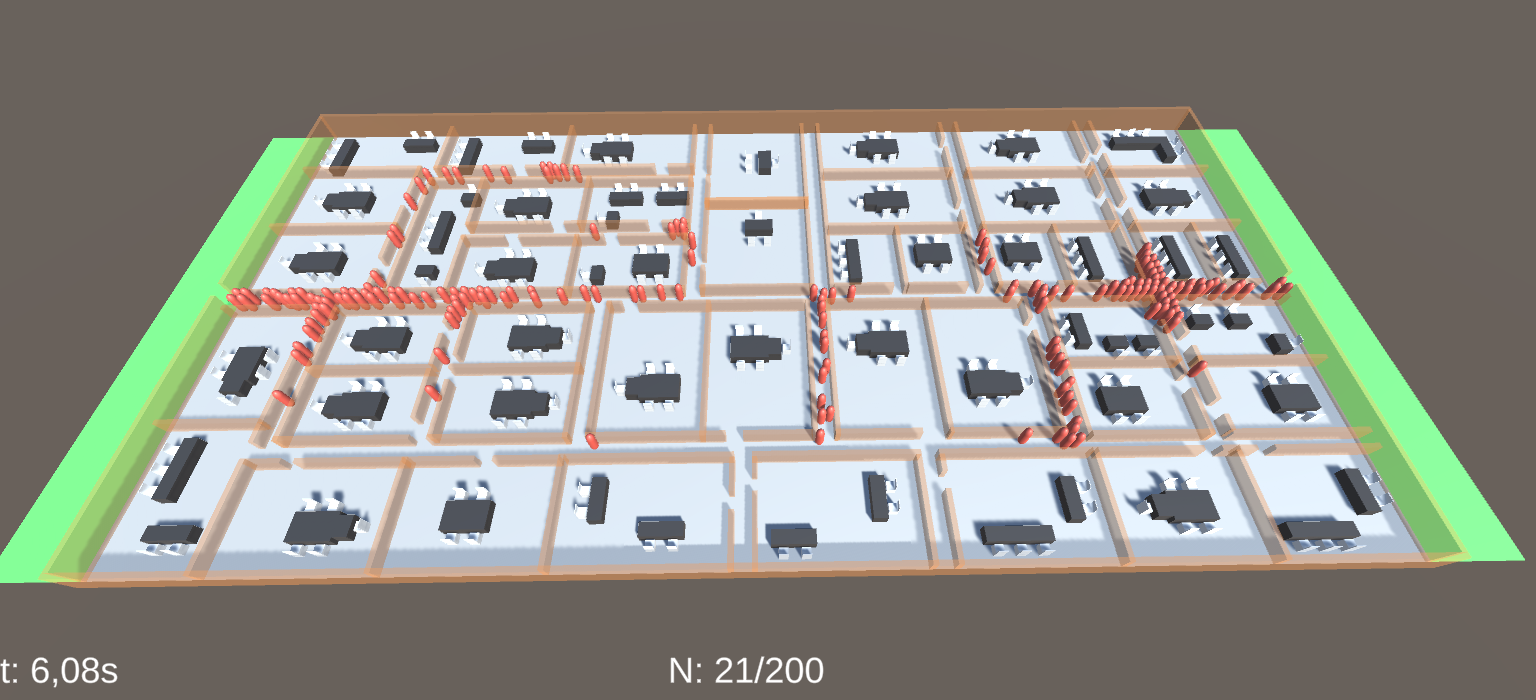
\includegraphics[scale=0.17]{4. carrefour.png}\newline
    $\hspace*{0.2cm}$- Je pense que le fait d'avoir plus de bureaux/couloirs a permis de bien diviser les flux ce qui a largement diminué les temps de sorties mais cela est atténué par les deux remarques précédentes.
    Donc certaines hypothèses pourront être tiré de cette simulation.

    \item Temps moyen de dernière sortie : 24.23
    \newline Temps max de dernière sortie : 34.37
    \newline Temps min de dernière sortie : 21.53
    \newline
    (Le temps moyen est meilleur que pour le 1., ce qui s'explique car il y a plus de couloir de circulation ce qui divise les flux)
    \newline\newline
    Certaines cloisons ont simplement été supprimé, les portes ont peu été modifié pour simplement montrer l'influence de la taille des bureaux et non de la disposition des portes.
    \newline
    $\hspace*{0.2cm}$- Un bureau possédant deux portes(situé à droite du milieu) sert maintenant de chemin de sortie ce qui diminue l'utilisation d'autre couloirs, cela semble avoir un effet positif.
    \newline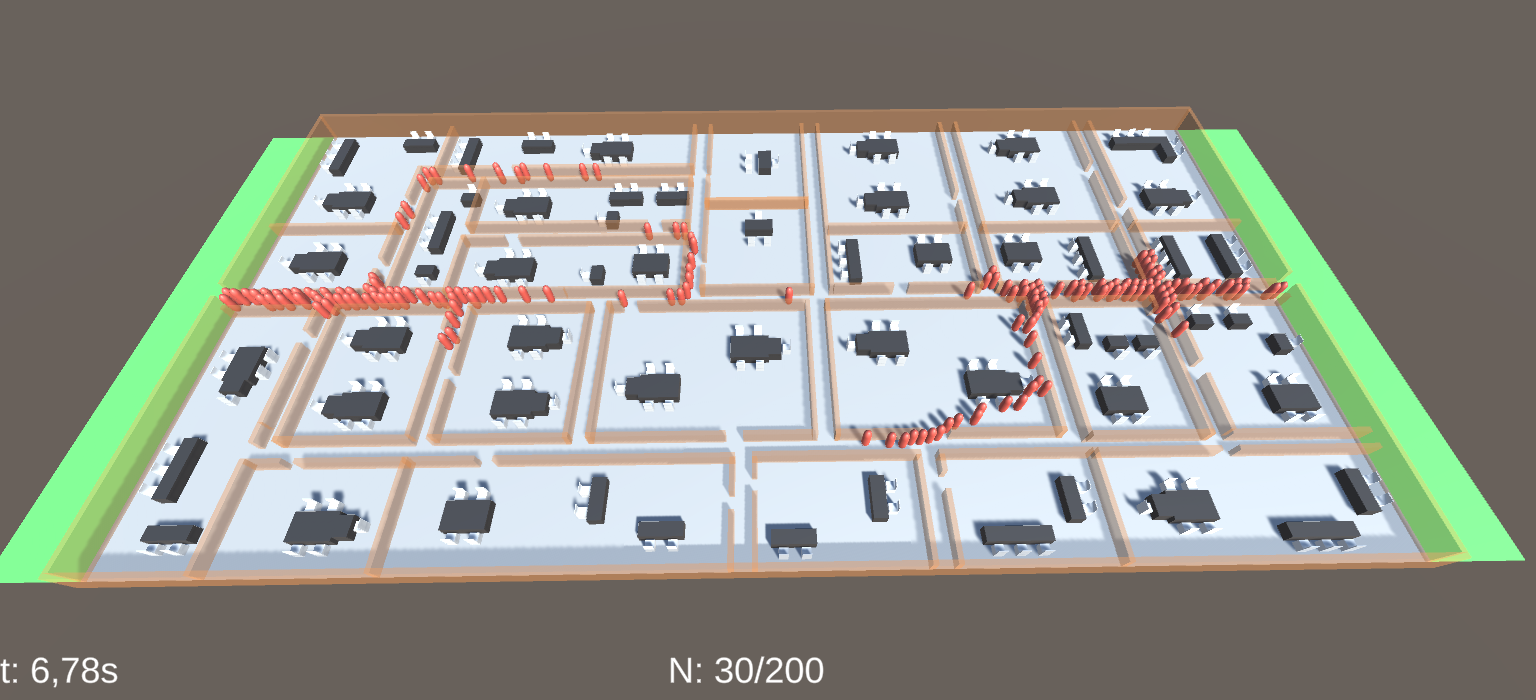
\includegraphics[scale=0.17]{5. nouveau chemin.png}\newline

    \item Temps moyen de dernière sortie : 23.84
    \newline Temps max de dernière sortie : 30.95
    \newline Temps min de dernière sortie : 20.36
    \newline
    (Meilleur temps moyen et minimale pour le moment, il semble que la destruction de certaines cloisons est entrainé de nouveaux axes de circulation et que les pièces
    restent encore assez petites pour que tous le monde n'emprunte pas les mêmes chemins.)
    \newline\newline
    Pareil que pour l'expérience précédente, je retire simplement des cloisons et laisse les portes a peu près dans la disposition où elles étaient.
    \newline
    $\hspace*{0.2cm}$- Il me semble qu'un grand objectif de l'optimisation semble apparaître, soit diviser le flux tout en offrant beaucoup de chemins possibles (sans tomber dans le piège d'avoir un seul chemin qui
    est toujours celui optimal et donc que les autres ne soit pas emprunté).
    \newline\newline\newline
    Pour les prochaines simulations (avec \textbf{1, 2 ou 3 portes}), l'idée n'est pas d'optimiser la location des portes (car je pense que cela joue en réalité un rôle crucial),
    mais simplement mettre le nombre de portes indiqué en essayant d'espacer au mieux les portes et de voir si simplement ajouter des portes a une influence sur le temps de sortie.
    (en sachant que certaines portes ne serront peut-être jamais emprunté si elles ne permettent pas d'acceder au meilleur chemin de sortie.)

    \item Temps moyen de dernière sortie : 23.72
    \newline Temps max de dernière sortie : 37.86
    \newline Temps min de dernière sortie : 18.64
    \newline
    (Meilleur temps moyen actuel, pire temps max, meilleur temps min (qui est d'ailleurs impressionant comparé aux autres))
    \newline
    Ici, peu de cloisons ont été modifiées en réalité, et les portes sont laissés comme elles étaient avant.
    \newline
    En faisant que de minimes changement, on a pu légèrement amélioré le temps, il y a deux explications possibles :
    \newline
    $\hspace*{0.2cm}$- Soit ça n'a rien changé et il n'y a pas eu assez de simulations mais cela aurait montré que c'était équivalent
    \newline
    $\hspace*{0.2cm}$- Soit il y a effectivement un petit changement, qui s'explique car de nouveaux chemins sont accesibles dans les bureaux, surtout pour le bureau entouré en vert sur la photo ci-dessous qui semble mieux ainsi.
    \newline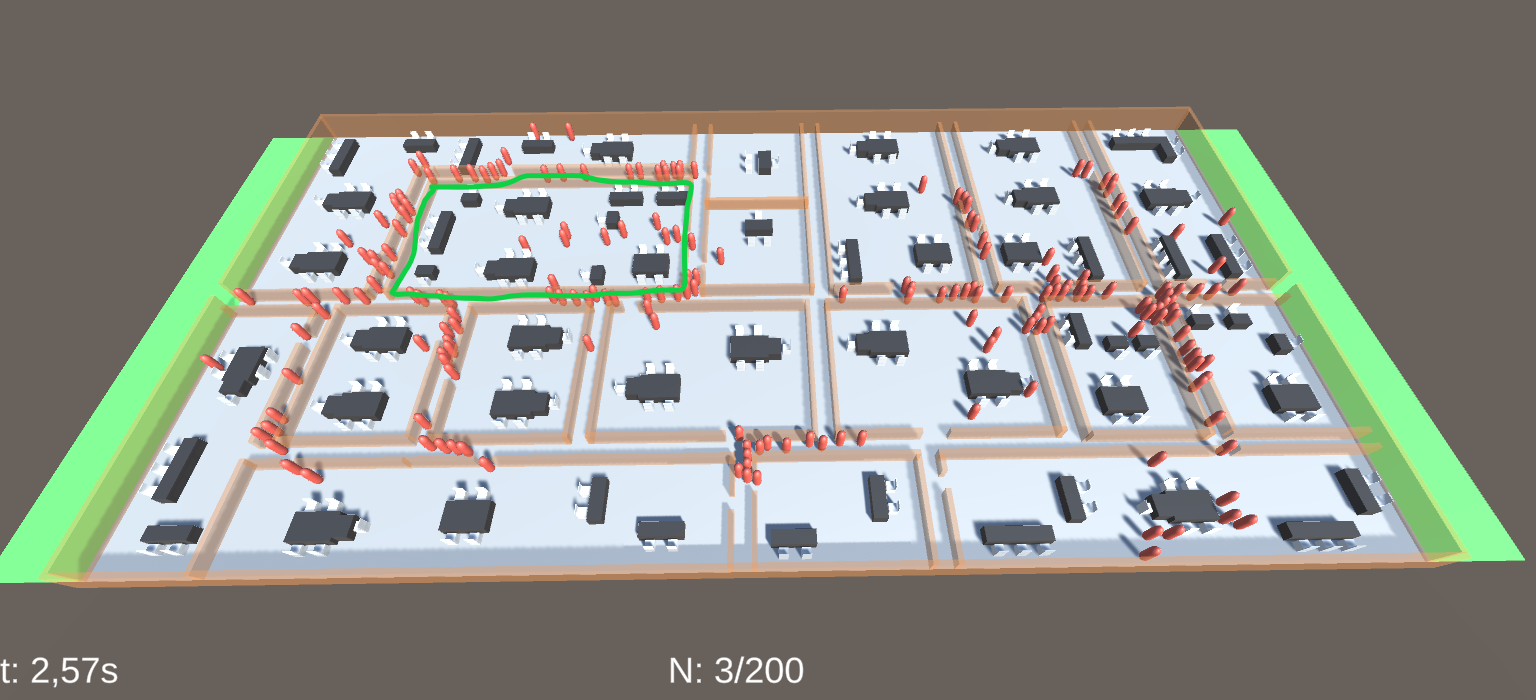
\includegraphics[scale=0.17]{7. bureaux amélioré.png}\newline
    \newline
    Ce qu'il faut retenir c'est qu'en effet le nombre de personnes par bureaux influe sur le temps de sortie, et en réalité pour diviser le flux il est parfois mieux de faire des bureaux de plus grande taille car cela fait que toutes les personnes
    de ce bureau se dirigeront vers la même porte, ce qui créera un petit flux au niveau de la porte de sortie mais permettra de ne pas avoir de bouchon avec les autres flux de personnes.
    \newline
    + le mieux n'est pas de grand bureau ni de petits (le 1. et le 4.) mais un mélange cohérent.




    \item Temps moyen de dernière sortie : 27.14
    \newline Temps max de dernière sortie : 34.26
    \newline Temps min de dernière sortie : 22.80
    \newline
    J'ai choisi de garder les structures du 7. car c'est celui proposant les meilleurs temps pour le moment. 
    \newline
    $\hspace*{0.2cm}$- Comme il n'y a qu'une porte par bureaux certains se retrouvent à devoir enormément marcher pour se diriger vers la sortie qu'ils ont choisit (ils doivent traverser tout le bureau pour arriver à la porte pour au final repartir dans l'autre
    sens, voir la photo et le chemin colorié que j'ai pu beaucoup observé.)
    \newline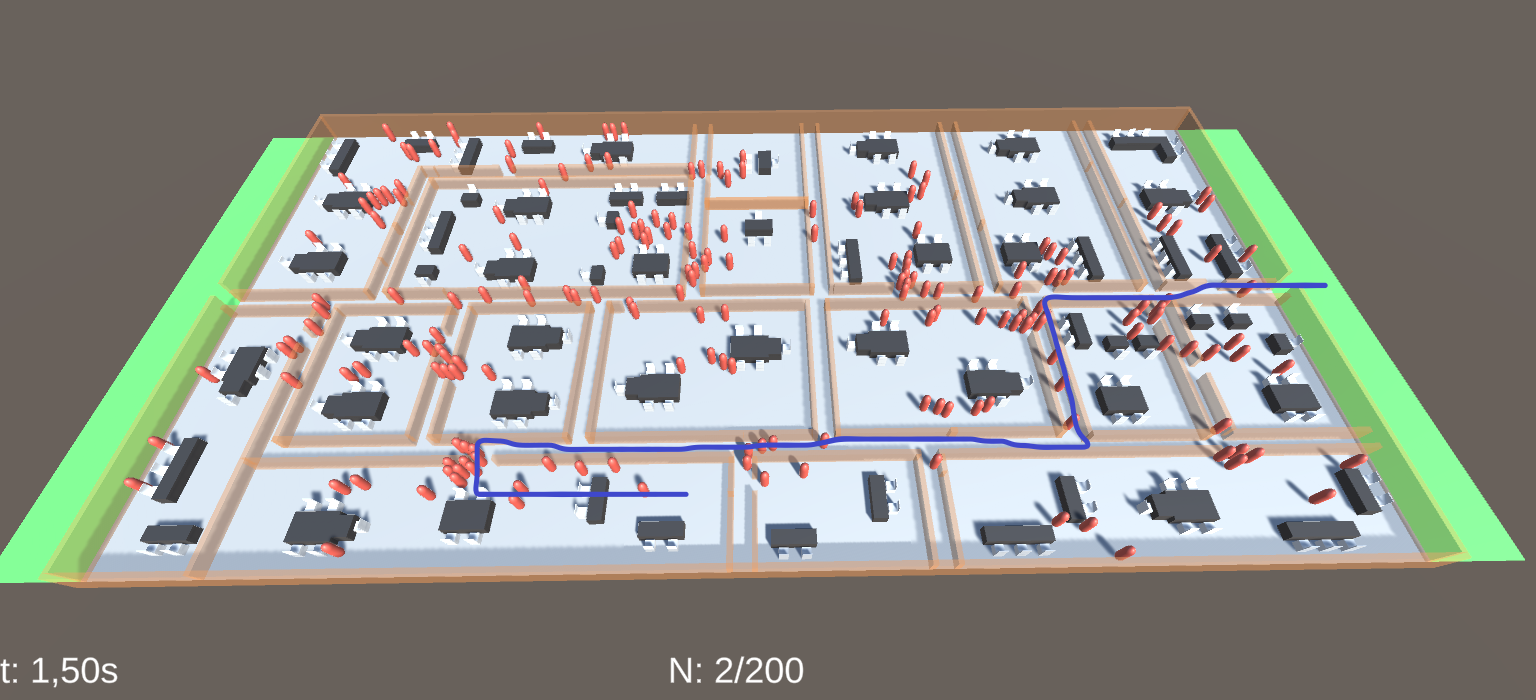
\includegraphics[scale=0.17]{8. chemin mauvais.png}\newline
    \newline
    $\hspace*{0.2cm}$- Un autre gros problème est le fait que les gens d'un même couloir veulent rejoindre des sorties opposés cela génère des concentrations importantes de personnes inutilement.
    \newline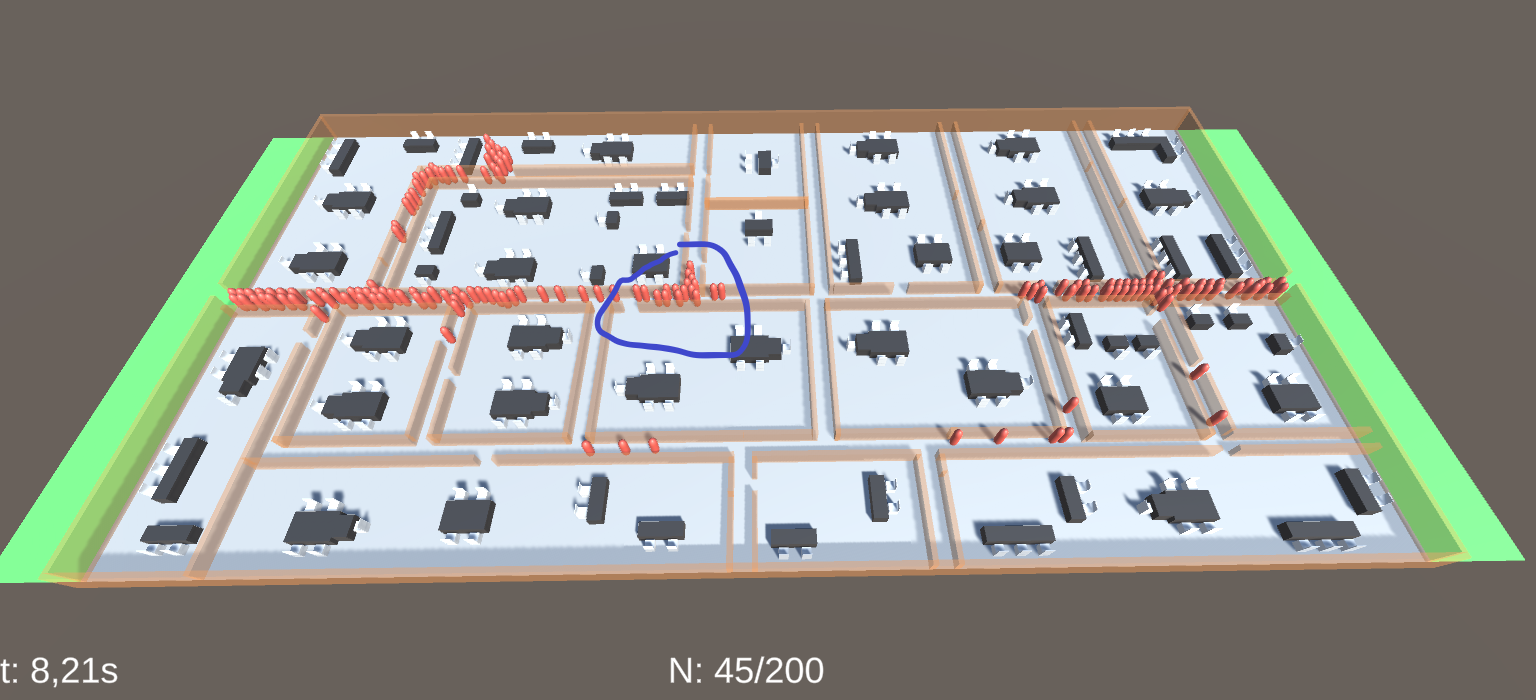
\includegraphics[scale=0.17]{8. collision.png}\newline
    Cela explique le temps obtenue qui n'est pas incroyable comparé au 7.

    \item Temps moyen de dernière sortie : 23.61
    \newline Temps max de dernière sortie : 32.17
    \newline Temps min de dernière sortie : 20.37
    \newline
    (Meilleur temps moyen, de peu loin par rapport au batiment 7., cela s'explique car il y a plus le carrefour qui provoquait un très grand flux, ce problème est cependant remplacer par un nouveau comme dit ensuite)
    \newline
    $\hspace*{0.2cm}$- Le plus gros problème réside dans le trop gros flux montré sur la photo. (Cela vient du fait que tous les chemins du bas menent à cette porte dans le bureau de droite donc le flux devient trop important
    à partir du milieu de la simulation et les personnes ne peuvent sortir car ceux dans le couloir principal prennent la priorité car ils sont en mouvement)
    \newline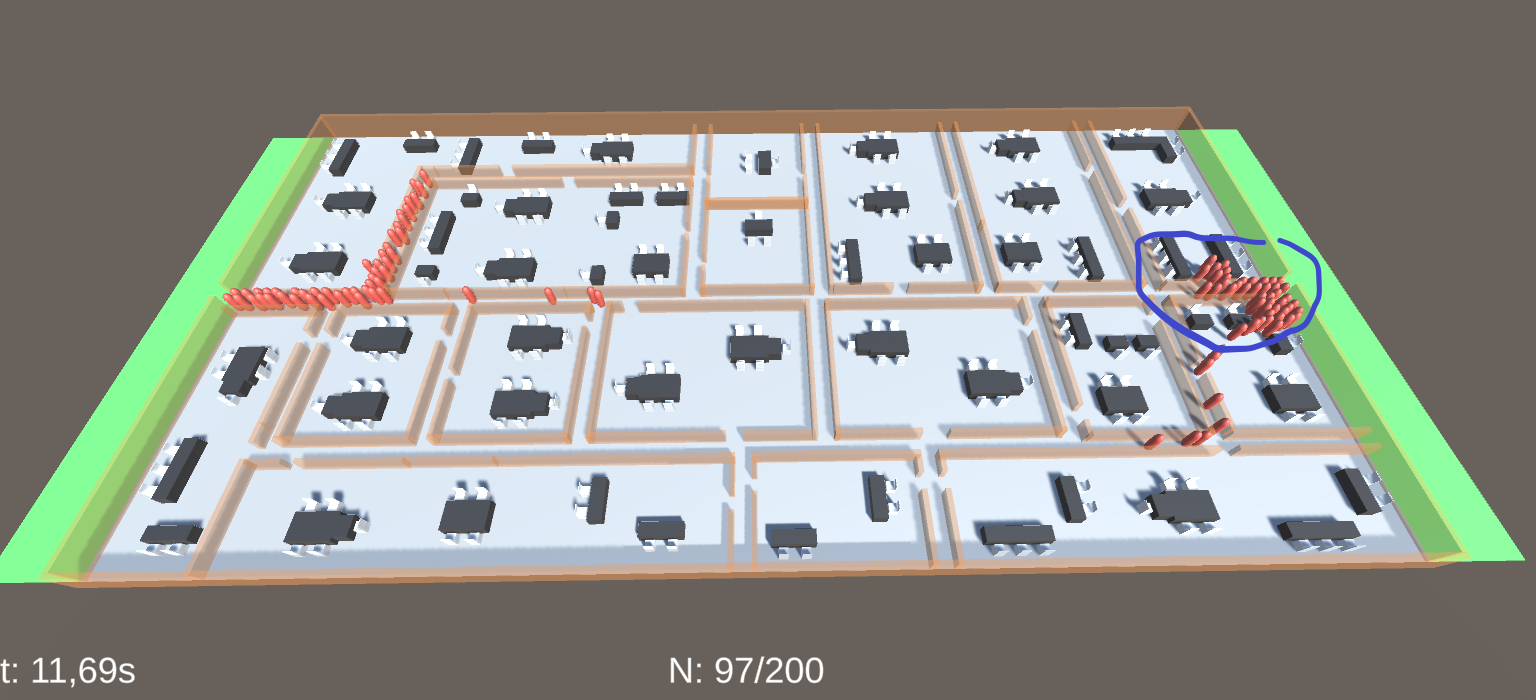
\includegraphics[scale=0.17]{9. blocage.png}\newline 

    \item Temps moyen de dernière sortie : 23.20
    \newline Temps max de dernière sortie : 28.86
    \newline Temps min de dernière sortie : 19.72
    \newline
    (Meilleurs temps moyen actuellement, expliqué par les points en dessous) 
    \newline
    $\hspace*{0.2cm}$-même majeur problème que pour le 9(au milieu à droite)
    \newline
    $\hspace*{0.2cm}$- un nouveau chemin s'est crée à gauche cependant reste à voir si il diminue ou non le temps de sortie
    \newline\newline
    Reste à tester avec 4 portes (j'aimerais montré qu'augmenter le nombre de portes indéfiniment n'améliorera pas le temps (on retournera à une situation proche de quand il n'y avait pas de mur sinon))

    \item (Bonus) 4 Portes par bureau
    \newline Temps moyen de dernière sortie : 27.87
    \newline Temps max de dernière sortie : 32.42
    \newline Temps min de dernière sortie : 23.42
    \newline
    (Cela confirme mes pensées, trop de portes est néfatse, car tout le monde finit par emprunter le même chemin au final)
    \newline
    $\hspace*{0.2cm}$- Voir l'image pour constater que tout le monde emprunte le même chemin ce qui créer d'important flux devant une porte et ralentit la sortie
    \newline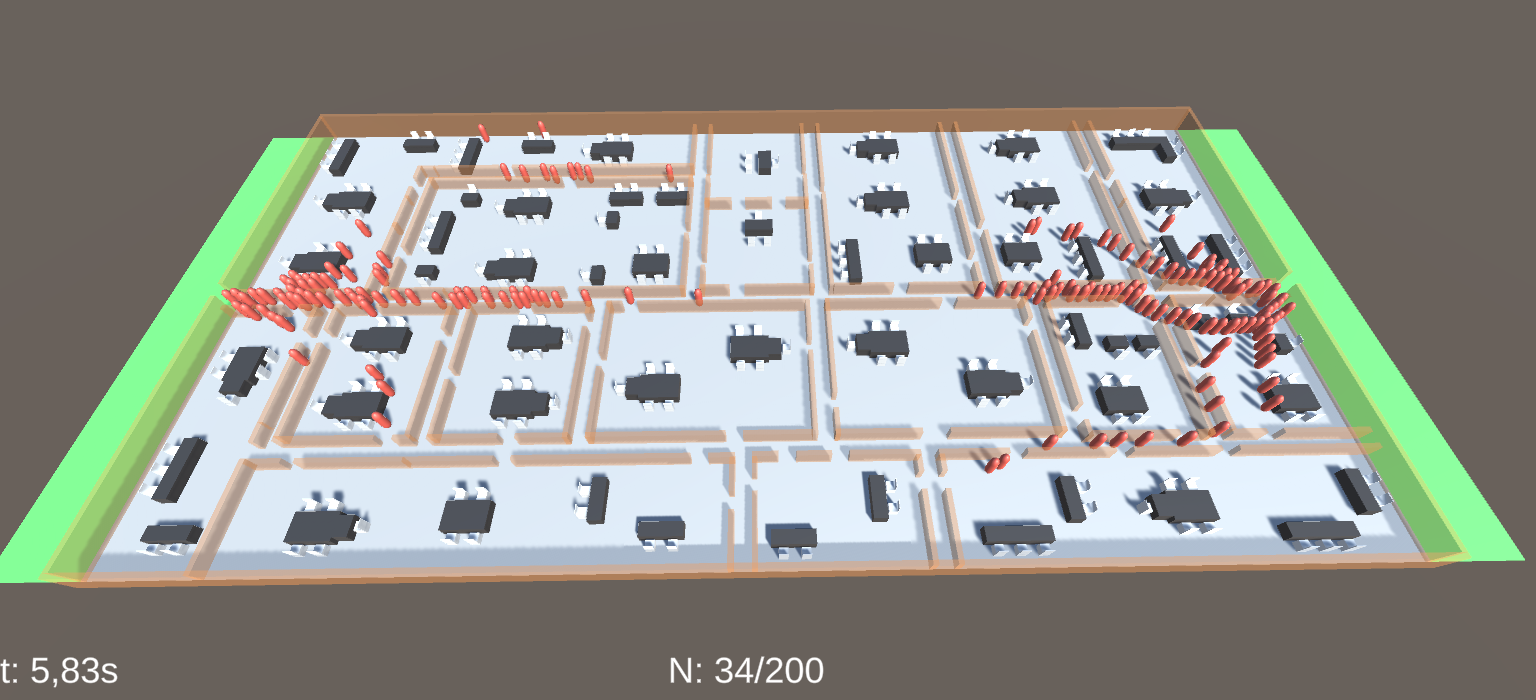
\includegraphics[scale=0.17]{11. chemin unique.png}\newline
\end{enumerate}

\end{document}